\documentclass[12pt]{article}
\usepackage{sbc-template}
\usepackage[utf8]{inputenc}
\usepackage[brazil]{babel}
\usepackage{graphicx,url,booktabs,amsmath}
\usepackage{fontspec}
\setmainfont{texgyretermes-regular.otf}[
  BoldFont=texgyretermes-bold.otf,
  ItalicFont=texgyretermes-italic.otf,
  BoldItalicFont=texgyretermes-bolditalic.otf]
\setsansfont{texgyreheros-regular.otf}[
  BoldFont=texgyreheros-bold.otf,
  ItalicFont=texgyreheros-italic.otf,
  BoldItalicFont=texgyreheros-bolditalic.otf]
\sloppy

\title{Avaliação de Desempenho de uma Rede Wi-Fi com Servidor Cabeado no ns-3}
\author{Diego Fontes de Avila\inst{1}, Gabriel Lopes Prodossimo\inst{1},
  João Victor Costa Teodoro\inst{1},\\ Matheus Davi Leão\inst{1},
  Sophia Soares Mariano\inst{1}}
\address{Equipe 6 -- PCS3614 Redes de Computadores I\\
  Escola Politécnica da Universidade de São Paulo (USP) -- São Paulo -- SP}

\begin{document}
\maketitle

\begin{abstract}
This report evaluates a wired-server/Wi-Fi-client topology in ns-3. We compare
static and walking clients, UDP, TCP and mixed transport, three application
patterns, and six client counts. Throughput, delay and packet loss are analyzed
from 108 reproducible simulation scenarios.
\end{abstract}

\begin{resumo}
Este trabalho avalia, no ns-3, uma rede com servidor cabeado e clientes Wi-Fi.
São comparados clientes estáticos e em caminhada aleatória, tráfego UDP, TCP e
misto, três padrões de aplicação e seis quantidades de clientes. Vazão, atraso
e perda são analisados em 108 cenários de simulação reproduzíveis.
\end{resumo}

\section{Introdução}
Redes locais sem fio compartilham o meio de transmissão. À medida que cresce
o número de estações, aumenta a disputa por acesso ao canal, e o desempenho
depende também do protocolo de transporte, do padrão de tráfego e da posição
dos dispositivos. Uma simulação de eventos discretos permite comparar essas
condições de forma controlada. O objetivo deste projeto é avaliar o impacto
da quantidade e da mobilidade dos clientes na comunicação com um servidor
cabeado, usando a topologia e as variações especificadas no enunciado
\cite{projeto}. Como referências gerais do simulador, consideram-se o guia
de instalação, o tutorial e a biblioteca de modelos da versão 3.43
\cite{instalacao,tutorial,modelos}.

\section{Descrição do exercício proposto}
A Figura~\ref{fig:topologia} apresenta a topologia implementada. O nó \(s2\)
é o servidor e ocupa a última posição lógica da LAN cabeada, na qual também
estão \(s0\), \(s1\) e o ponto de acesso (AP). O AP liga o segmento CSMA
\texttt{10.1.1.0/24} à rede Wi-Fi \texttt{192.168.0.0/24}, com SSID
\texttt{Equipe6}. Cada cliente \(c_i\) conecta-se ao AP e recebe dados
originados no servidor; os nós \(s0\) e \(s1\) integram a topologia cabeada,
mas não geram aplicações. O roteamento IP é configurado automaticamente.

\begin{figure}[ht]
  \centering
  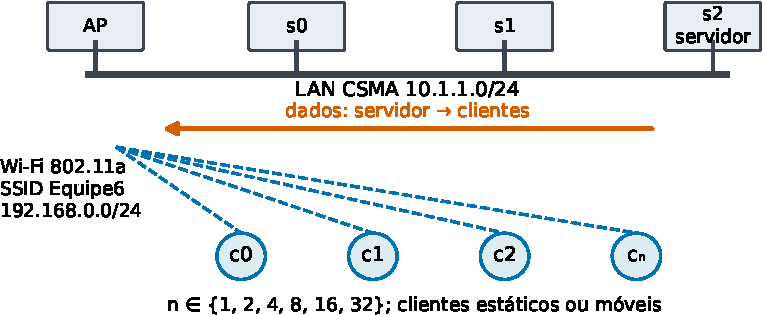
\includegraphics[width=.98\textwidth]{figuras/topologia.pdf}
  \caption{Topologia e sentido do tráfego de aplicação. A LAN é um meio CSMA compartilhado, e o AP conecta o servidor aos clientes sem fio.}
  \label{fig:topologia}
\end{figure}

\section{Avaliação de desempenho}
\subsection{Metodologia}
A implementação usa ns-3 3.44 \cite{ns3} com interface Python 3.10.12 e o modelo Wi-Fi
Yans para IEEE 802.11a. O servidor instala uma aplicação \texttt{OnOff} por
cliente; cada cliente instala seu próprio \texttt{PacketSink}. As fontes
iniciam aproximadamente em \(t=4\)~s, terminam em \(t=58\)~s e os receptores
ficam ativos desde \(t=1\)~s. No modo CBR, a aplicação permanece ativa; na
rajada, alterna 1~s ativa e 1~s inativa. No modo CBR/Rajada, os clientes de
índice par usam CBR e os de índice ímpar usam rajada.

Foram executadas as \(2\times3\times3\times6=108\) combinações de mobilidade,
transporte, aplicação e número de clientes. Para \(n\geq2\), o modo misto
divide igualmente os clientes entre UDP e TCP. Com \(n=1\), uma divisão
50\%/50\% é impossível; o único cliente usa UDP. Cada combinação foi executada
uma vez, por 60~s simulados, com semente 6 e número de rodada definido pela
combinação; o contador de fluxos aleatórios do ns-3 é reiniciado a cada
cenário, de modo que o resultado não depende da ordem de execução. Não são apresentados intervalos de confiança: as comparações são
descritivas desta realização, não estimativas estatísticas de múltiplas
sementes. No caso misto com dois clientes e padrão CBR/Rajada, os protocolos
coincidem com padrões distintos; essa combinação não isola o efeito de cada
fator.

Os clientes estáticos permanecem em posições fixas; os móveis partem das
mesmas posições e, mantendo 1 ou 2~m/s, sorteiam uma nova direção a cada 2~s.
Se o próximo deslocamento ultrapassaria a borda, a componente da velocidade
correspondente é invertida antes do passo. A velocidade entre mudanças é implementada por
\texttt{ConstantVelocityMobilityModel} \cite{mobility}. Os clientes iniciam em uma malha na
região central, dentro da área de 140~m \(\times\) 140~m. Cada cliente móvel
tem um fluxo pseudoaleatório próprio, reproduzível pela semente e pela rodada.

Os experimentos foram executados em Ubuntu 22.04.5 LTS sob WSL2, em uma
máquina com Intel Core i5-12450H (12 núcleos lógicos) e 3,7~GiB de
memória disponibilizada ao ambiente. Até três processos independentes
rodaram cenários em paralelo; isso reduz o tempo de execução real, sem alterar
os 60~s de tempo simulado nem os resultados de cada cenário.

\subsection{Parâmetros e métricas}
\begin{table}[ht]
\centering\small
\caption{Parâmetros efetivamente usados nos experimentos.}
\label{tab:parametros}
\begin{tabular}{ll}
\toprule
Parâmetro & Valor \\
\midrule
Duração e janela de tráfego & 60~s; 4--58~s (54~s) \\
Clientes & 1, 2, 4, 8, 16 e 32 \\
Área e posições iniciais & 140~m \(\times\) 140~m; região central \\
Wi-Fi, SSID e antenas do AP & IEEE 802.11a; Equipe6; 1 \\
Potência Wi-Fi & 16~dBm \\
LAN cabeada & CSMA, 100~Mbit/s; 10~\(\mu\)s \\
Mobilidade estática & 0~km/h; ConstantPositionMobilityModel \\
Mobilidade móvel & 3,6 ou 7,2~km/h; nova direção a cada 2~s \\
Taxa da aplicação por cliente & 512~kbit/s durante o período ativo \\
Dados por envio UDP/TCP & 512/1500~bytes, sem contar cabeçalhos \\
Aplicações & CBR, Rajada (1~s/1~s), CBR/Rajada \\
Transportes & UDP, TCP, metade UDP/metade TCP \\
\bottomrule
\end{tabular}
\end{table}

As métricas foram extraídas com \texttt{FlowMonitor} nos fluxos de dados
servidor\(\rightarrow\)cliente, excluindo fluxos reversos de ACK TCP
\cite{flowmonitor}. A vazão agregada é \(8\sum_i B_{i,\mathrm{rx}}/(54\cdot
10^6)\) Mbit/s, usando bytes IP recebidos. O atraso é a média de
\texttt{delaySum/rxPackets}, ponderada pelo número de pacotes recebidos. A
perda é \(100\,\sum_i(\mathrm{txPackets}_i-\mathrm{rxPackets}_i)/
\sum_i\mathrm{txPackets}_i\). O jitter médio é calculado a partir de
\texttt{jitterSum/(rxPackets-1)}, ponderado pelos pares de pacotes recebidos.
A justiça de Jain usa as vazões individuais: \(J=(\sum_i v_i)^2/
(n\sum_i v_i^2)\). Os CSVs registram ainda contadores de pacotes e bytes
enviados e recebidos, entrega e vazão média por cliente. Essas métricas são
da camada IP: a vazão inclui cabeçalhos;
as contagens TCP podem incluir retransmissões, e a perda aqui não é a perda
final percebida pela aplicação.

\section{Resultados}
As Figuras~\ref{fig:vazao}--\ref{fig:perda} mostram todas as 108 combinações.
Cada linha de painéis representa um padrão de aplicação, cada coluna uma
condição de mobilidade e cada curva um transporte. Os valores numéricos
completos constam dos arquivos \texttt{resumo.csv} e \texttt{fluxos.csv}.

\subsection{Vazão e carga oferecida}
O padrão de aplicação explica a tendência principal da vazão
(Figura~\ref{fig:vazao}). Com 32 clientes, a oferta de dados de aplicação é
16,384~Mbit/s em CBR, aproximadamente 8,192~Mbit/s em rajada e
12,288~Mbit/s em CBR/Rajada. No UDP estático, as vazões IP recebidas foram,
respectivamente, 16,757, 8,624 e 12,954~Mbit/s. Os valores IP podem exceder
a taxa de dados da aplicação porque incluem cabeçalhos. A LAN cabeada de
100~Mbit/s comporta essas ofertas; a disputa e o enfileiramento tendem a se
concentrar no único rádio do AP. Essa é uma interpretação da topologia, não
uma medição direta da ocupação do canal.

O aumento de carga nem sempre se traduz imediatamente em perda: no UDP/CBR
estático com 32 clientes, 97,0\% dos pacotes chegaram, mas o atraso médio já
era 159,9~ms. No UDP/Rajada estático com 32 clientes, o atraso foi 16,8~ms e
a perda, 0,1\%. Pacotes que aguardam acesso ao meio ainda podem ser entregues,
e a alternância entre períodos ativos e inativos reduz a oferta média. O
CBR/Rajada estático obteve atraso de 12,4~ms apesar da oferta média maior que
a rajada pura; uma explicação compatível é que a combinação distribui parte
da carga continuamente, enquanto as rajadas de clientes sincronizados geram
picos simultâneos. Não foram coletados rastros de fila para confirmar essa
hipótese.

\begin{figure}[p]
  \centering
  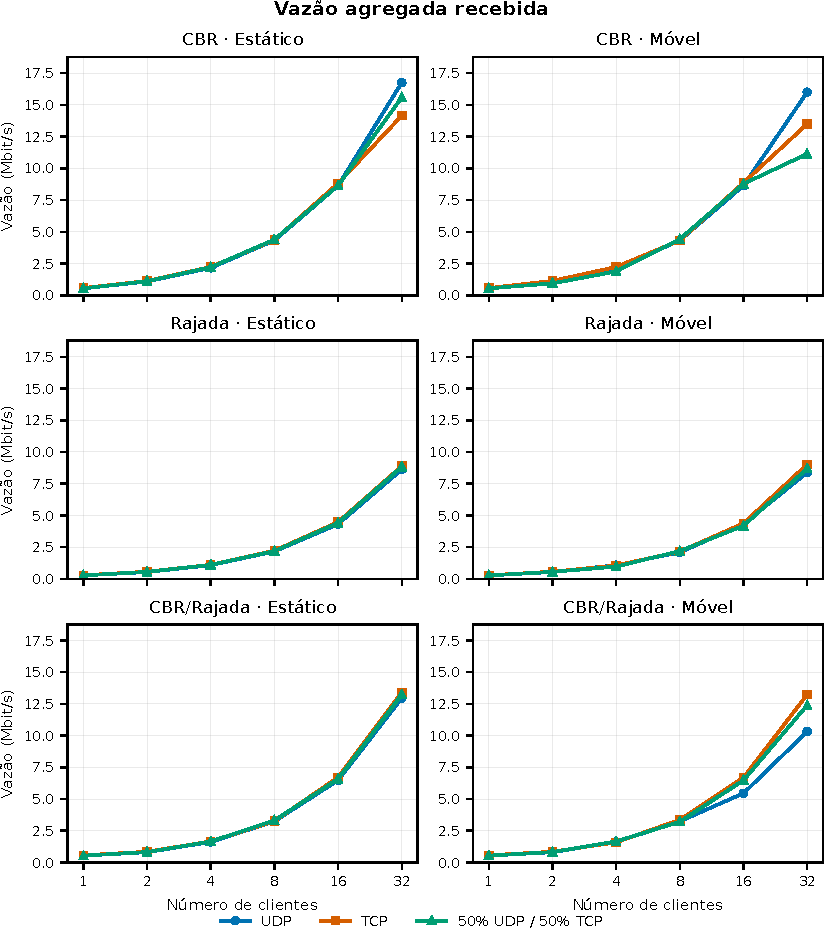
\includegraphics[width=.96\textwidth]{figuras/vazao.pdf}
  \caption{Vazão IP agregada em função do número de clientes.}
  \label{fig:vazao}
\end{figure}

\begin{figure}[p]
  \centering
  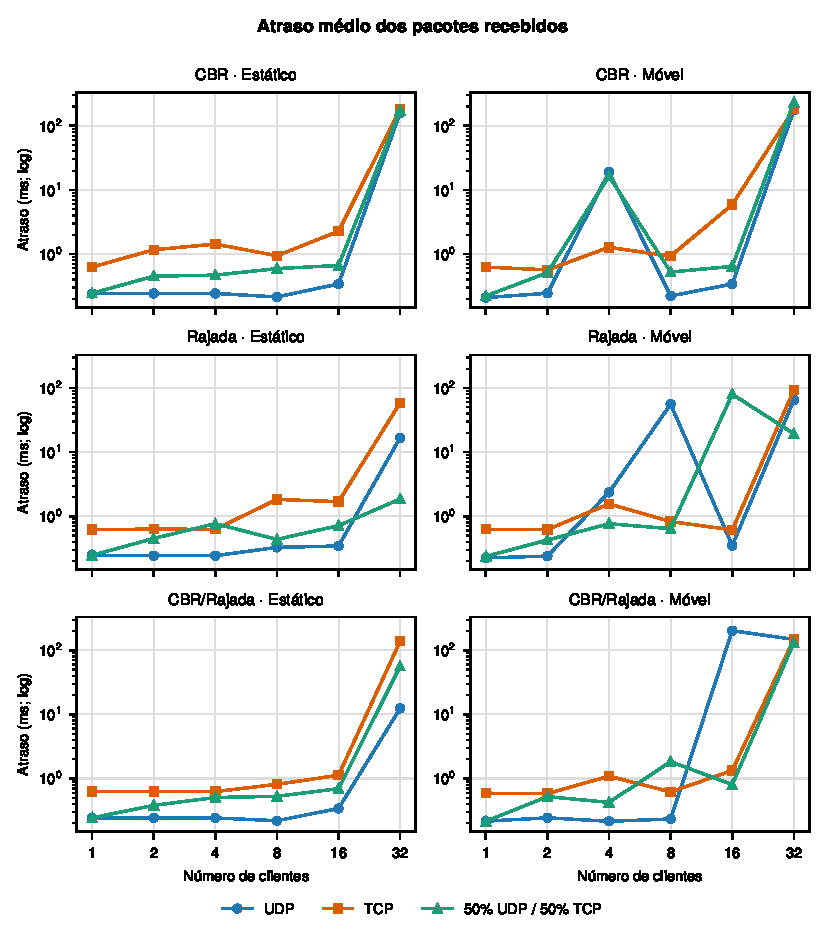
\includegraphics[width=.96\textwidth]{figuras/atraso.pdf}
  \caption{Atraso médio dos pacotes IP entregues. O eixo vertical usa escala logarítmica, para representar tanto submilissegundos quanto centenas de milissegundos.}
  \label{fig:atraso}
\end{figure}

\begin{figure}[p]
  \centering
  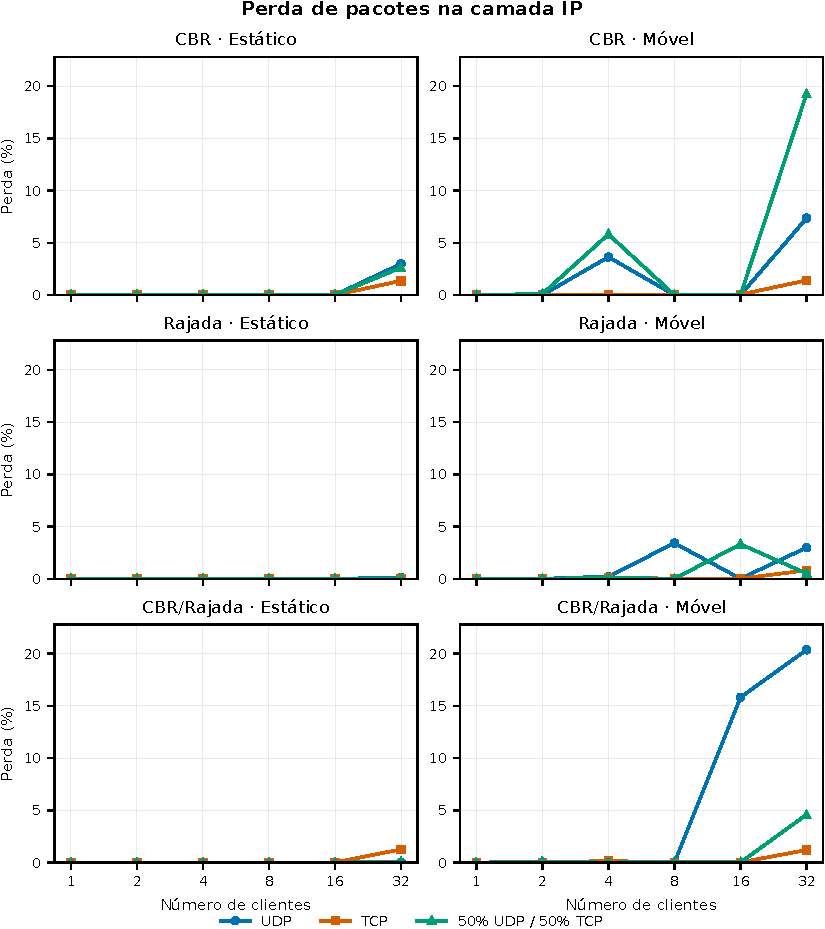
\includegraphics[width=.96\textwidth]{figuras/perda.pdf}
  \caption{Fração de pacotes IP transmitidos que não chegaram ao destino. Em TCP, retransmissões podem contribuir para as contagens.}
  \label{fig:perda}
\end{figure}
\clearpage

\subsection{Discussão dos resultados}
A mobilidade teve efeito variável (Figuras~\ref{fig:atraso} e
\ref{fig:perda}). Em UDP/CBR-Rajada com 32 clientes, a vazão caiu de 12,954
para 10,313~Mbit/s, a perda subiu de aproximadamente zero para 20,4\% e o
atraso passou de 12,4 para 148,0~ms. No CBR misto com 32 clientes, a entrega
caiu de 97,3\% para 80,5\%, e o atraso aumentou de 172,7 para 232,3~ms.
O deslocamento altera distâncias ao AP e condições de propagação; junto à
contenção pelo canal, isso é compatível com as degradações observadas.
Entretanto, trajetórias diferentes e uma única rodada por combinação impedem
atribuir com certeza cada diferença somente à mobilidade.

O TCP não eliminou atrasos: em CBR com 32 clientes, o atraso foi 183,7~ms no
estático e 181,6~ms no móvel, embora a perda IP tenha ficado em 1,2\% e
1,5\%, respectivamente. Retransmissões, confirmações e controle de fluxo influenciam tanto a
vazão quanto as contagens de pacotes IP. Entre os indicadores adicionais, o
jitter médio em TCP/Rajada com 32 clientes cresceu de 2,1~ms no estático para
3,9~ms no móvel. A justiça de Jain foi 0,878 no UDP/CBR-Rajada móvel com
32 clientes. Nesse padrão, porém, os clientes já possuem ofertas distintas;
um índice inferior a um não prova, isoladamente, distribuição injusta do
canal. Os dados não incluem rastros MAC/PHY nem repetições com outras
sementes, de modo que os mecanismos propostos permanecem explicações
plausíveis, não causas isoladas experimentalmente.

\section{Detalhamento da divisão do trabalho}
A Tabela~\ref{tab:divisao} resume a contribuição de cada integrante. As
funções correspondentes do script estão identificadas no próprio código.

\begin{table}[ht]
\centering\small
\caption{Divisão do trabalho entre os integrantes da equipe.}
\label{tab:divisao}
\begin{tabular}{lp{.62\textwidth}}
\toprule
Integrante (NUSP) & Atividades \\
\midrule
Diego F. de Avila (15447910) & Instalação do ns-3; LAN CSMA, endereços IP e roteamento \\
Gabriel L. Prodossimo (15453560) & Wi-Fi 802.11a (AP, SSID, potência) e caminhada aleatória \\
João Victor C. Teodoro (15463850) & Aplicações UDP, TCP e mista; padrões CBR e rajada \\
Matheus D. Leão (15520593) & FlowMonitor, métricas, execução dos 108 cenários e CSVs \\
Sophia S. Mariano (15511213) & Gráficos, figura da topologia, redação e revisão do relatório \\
\bottomrule
\end{tabular}
\end{table}

\section{Conclusão}
Os 108 cenários permitiram observar o efeito conjunto da carga, do protocolo
de transporte e da caminhada aleatória sobre os clientes Wi-Fi atendidos por
um servidor cabeado. O padrão de aplicação determina a oferta média; em alta
carga, o atraso pode crescer mesmo com entrega elevada. A mobilidade produziu
quedas expressivas em algumas combinações, mas não uniformemente, e o TCP
apresentou baixa perda IP sem garantir baixo atraso. Os resultados descrevem
uma execução reproduzível por combinação; rodadas adicionais e rastreamento
MAC/PHY seriam necessários para estimar variabilidade e isolar causas.

\begin{thebibliography}{9}
\bibitem{projeto} PCS3614. \emph{Instruções do Projeto, 3º quadrimestre de 2026}.
Documento da disciplina, Universidade de São Paulo, 2026.
\bibitem{ns3} ns-3 Consortium. \emph{ns-3 Documentation}. Disponível em:
\url{https://www.nsnam.org/documentation/}. Acesso em: 1 nov. 2026.
\bibitem{instalacao} ns-3 Consortium. \emph{ns-3 Installation Guide}, versão 3.43.
Disponível em: \url{https://www.nsnam.org/docs/release/3.43/installation/ns-3-installation.pdf}.
Acesso em: 1 nov. 2026.
\bibitem{tutorial} ns-3 Consortium. \emph{ns-3 Tutorial}, versão 3.43.
Disponível em: \url{https://www.nsnam.org/docs/release/3.43/tutorial/ns-3-tutorial.pdf}.
Acesso em: 1 nov. 2026.
\bibitem{modelos} ns-3 Consortium. \emph{ns-3 Model Library}, versão 3.43.
Disponível em: \url{https://www.nsnam.org/docs/release/3.43/models/ns-3-model-library.pdf}.
Acesso em: 1 nov. 2026.
\bibitem{flowmonitor} ns-3 Consortium. \emph{Flow Monitor: Model Library}.
Disponível em: \url{https://www.nsnam.org/docs/models/html/flow-monitor.html}.
Acesso em: 1 nov. 2026.
\bibitem{mobility} ns-3 Consortium. \emph{Mobility: Model Library}.
Disponível em: \url{https://www.nsnam.org/docs/models/html/mobility.html}.
Acesso em: 1 nov. 2026.
\end{thebibliography}

\end{document}
